%
% trafo.tex
%
% (c) 2019 Prof Dr Andreas Müller, Hochschule Rapperswil
%

\def\curve#1#2#3{
\begin{scope}
\clip (-6.5,-3) rectangle (6.5,3);
\draw[line width=1pt,color=red]
	plot[domain={((#2)-2*abs(#1))}:{((#2)+2*abs(#1))},samples=100]
	({\x},{(#3)*sin(8*((\x-(#2))/(#1))*(180/3.1415))*exp(-((\x-(#2))/(#1))*((\x-(#2))/(#1)))/sqrt(abs(#1))});
\end{scope}
}

\def\flaeche#1#2#3{
\begin{scope}
\clip (-6.5,-3) rectangle (6.5,3);
\fill[color=red!20]
	plot[domain={((#2)-2*abs(#1))}:{((#2)+2*abs(#1))},samples=200]
	({\x},{(#3)*exp(-((\x-(#2))/(#1))*((\x-(#2))/(#1)))/sqrt(abs(#1))})
	--
	plot[domain={((#2)+2*abs(#1))}:{((#2)-2*abs(#1))},samples=200]
	({\x},{-(#3)*exp(-((\x-(#2))/(#1))*((\x-(#2))/(#1)))/sqrt(abs(#1))})
	--cycle;
\end{scope}
}

\def\achsen#1{
	\draw[->,line width=0.7pt] (-6.6,0)--(7.0,0) coordinate[label={$t$}];
	\draw[->,line width=0.7pt] (0,{-#1})--(0,{#1});
	\foreach \x in {1,...,6}{
		\draw[line width=0.7pt] ({\x},-0.08)--({\x},0.08);
		\draw[line width=0.7pt] ({-\x},-0.08)--({-\x},0.08);
	}
}

\def\cwt#1#2#3{
	\draw[->,line width=0.7pt]
		(-6.6,{#3-2})--(7.0,{#3-2}) coordinate[label={$b$}];
	\draw[->,line width=0.7pt]
		(0,{#3-2.1})--(0,{#3+0.4}) coordinate[label={left:$a$}];
	\fill[color=red] ({#2},{#3-2+#1}) circle[radius=0.08];
}

%\subsection{Das Gabor-Wavelet}
\rhead{Gabor / Heisenberg}
\begin{figure}
	\centering
	\includegraphics{papers/complex/images/gabor.pdf}
	\caption{Das Gabor-Wavelet für $\sigma = 2\pi$ \label{complex:gabor}}
\end{figure}

Die schlechte Lokalisierung des Haar-Wavelets in der Frequenz ist schon in seinem Spektrum ersichtlich.
Die Frequenzen neben $\omega_\psi$ fallen nur langsam ab.
Durch Heisenberg (Satz~\ref{satz:heisenberg}) wissen wir, dass die beste Lokalisierung durch Gaus-Funktionen erreicht wird.
Als nächstes verwenden wir deshalb das Gabor-Wavelet
\[
	\psi_\text{Gabor} = c_\sigma e^{-\frac{t^2}{2}}\left(\cos\left(\sigma t\right) - \kappa_\sigma\right),
\]
welches in Abbildung~\ref{complex:gabor} ersichtlich ist.
$c_\sigma$ und $\kappa_\sigma$ sind hierbei positive, reelle Konstanten.
$c_\sigma$ korrigiert die Norm des Wavelets, so dass $\|\psi\| = 1$.
$\kappa_\sigma$ ist notwendig für die Zulässigkeitsbedingung~\eqref{cwt:zulaessig}, welche u.~A.~fordert, dass das Integral des Wavelets verschwindet,  $\int_{-\infty}^{\infty}\psi\,\mathrm{d}t = 0$.
$\kappa_\sigma$ ist typischerweise sehr klein und wird in der Numerik oftmals einfach weggelassen.

$\sigma$ erlaubt es, Zeit- und Frequenz-Lokalisierung gegeneinander abzuwägen.
Die dominante Frequenz $\omega_\psi$ dieses Wavelets ist für $5 < \sigma \approx \omega_\psi$.
Das Gabor-Wavelet eignet sich deshalb besonders gut, um einzelne Frequenzen in einem Signal zu finden.
Betrachten wir die Wavelet-Transformierten unserer Beispielsignale mit dem Gabor-Wavelet in Abbildung~\ref{complex:gabor-ex}.

% CWT mit Haar-Wavelet hier, da sonst Gabor-Wavelet zu weit runter rutscht
\begin{figure}
	\centering
	\includegraphics{papers/complex/images/chirp_haar.pdf}
	\includegraphics{papers/complex/images/square_haar.pdf}
	\caption{Farb-codierte Wavelet-Transformationen der beiden Beispielsignale mit dem Haar-Wavelet.}
	\label{complex:haar-ex}
\end{figure}
\begin{figure}
	\centering
	\includegraphics{papers/complex/images/chirp_gabor.pdf}
	\includegraphics{papers/complex/images/square_gabor.pdf}
	\caption{Farb-codierte Wavelet-Transformationen  der beiden Beispielsignale mit dem Gabor-Wavelet.}
	\label{complex:gabor-ex}
\end{figure}

Auch hier ist die Signalfrequenz als Schwingung in der Amplitude ersichtlich. 
Die Lokalisierung in der Frequenz ist deutlich besser und die Verschiebung zwischen $a$ und $f$ klein, allerdings fliessen die Frequenzsprünge ineinander über, statt wie beim Haar-Wavelet scharf getrennt zu sein.
Durch die Wahl von $\sigma$ kann die Form des Wavelets angepasst werden und bietet folglich etwas Freiheit.
Wie auch beim Haar-Wavelet ist die Phase und die Amplitude nicht separierbar.
Auch hier finden wir die charakteristische Schwingung in der Amplitude wieder.
Diesem Problem wenden wir uns nun zu.

%%
% tikztemplate.tex -- template for standalon tikz images
%
% (c) 2019 Prof Dr Andreas Müller, Hochschule Rapperswil
%
\documentclass[tikz]{standalone}
\usepackage{amsmath}
\usepackage{times}
\usepackage{txfonts}
\usepackage{pgfplots}
\usepackage{csvsimple}
\usetikzlibrary{arrows,intersections,math}
\begin{document}
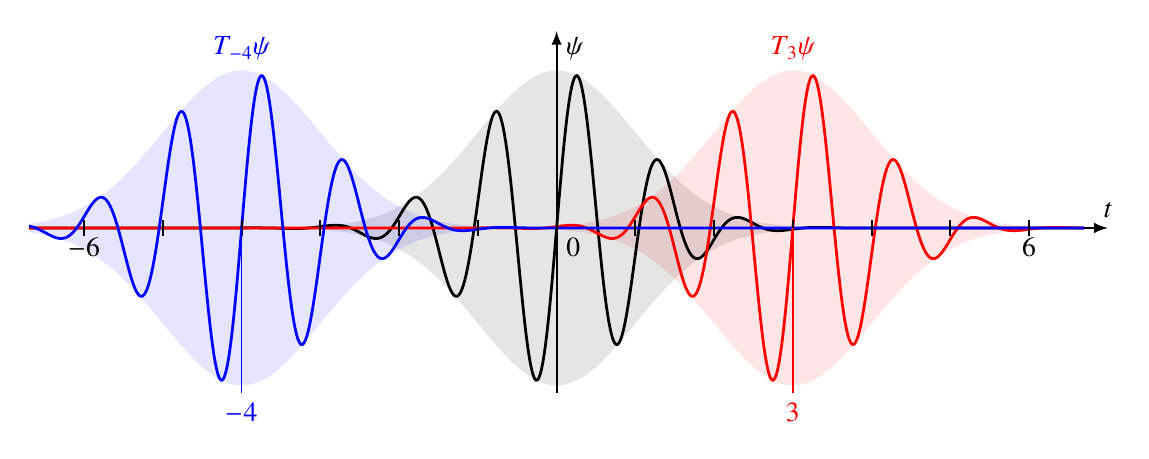
\begin{tikzpicture}[>=latex]

\def\pivalue{3.14159}
\def\frequency{6}

\fill[color=gray!20] 
	plot[domain=-4:4,samples=200]
		({\x},{2*exp(-(\x*\x/2))}) --
	plot[domain=4:-4,samples=200]
		({\x},{-2*exp(-(\x*\x/2))})
	--cycle;

\def\offsetone{3}
\fill[color=red!10] 
	plot[domain={\offsetone-4}:{\offsetone+4},samples=200]
		({\x},{2*exp(-((\x-\offsetone)*(\x-\offsetone)/2))}) --
	plot[domain={\offsetone+4}:{\offsetone-4},samples=200]
		({\x},{-2*exp(-((\x-\offsetone)*(\x-\offsetone)/2))})
	--cycle;

\node[color=red] at ({\offsetone},2) [above] {$T_{\offsetone}\psi$};
\definecolor{redgray}{rgb}{0.9,0.8,0.8}
\fill[color=redgray]
	plot[domain={\offsetone-4}:{\offsetone/2},samples=100]
		({\x},{2*exp(-((\x-\offsetone)*(\x-\offsetone)/2))}) --
	plot[domain={\offsetone/2}:4,samples=100]
		({\x},{2*exp(-(\x*\x/2))}) --
	plot[domain=4:{\offsetone/2},samples=100]
		({\x},{-2*exp(-(\x*\x/2))}) --
	plot[domain={\offsetone/2}:{\offsetone-4},samples=100]
		({\x},{-2*exp(-((\x-\offsetone)*(\x-\offsetone)/2))}) -- cycle;

\def\offsetone{-4}
\fill[color=blue!10] 
	plot[domain=-6.7:{\offsetone+4},samples=200]
		({\x},{2*exp(-((\x-\offsetone)*(\x-\offsetone)/2))}) --
	plot[domain={\offsetone+4}:-6.7,samples=200]
		({\x},{-2*exp(-((\x-\offsetone)*(\x-\offsetone)/2))})
	--cycle;
\node[color=blue] at ({\offsetone},2) [above] {$T_{\offsetone}\psi$};
\definecolor{bluegray}{rgb}{0.8,0.8,0.9}
\fill[color=bluegray]
	plot[domain=-6.7:{\offsetone/2},samples=100]
		({\x},{2*exp(-(\x*\x/2))}) --
	plot[domain={\offsetone/2}:4,samples=100]
		({\x},{2*exp(-((\x-\offsetone)*(\x-\offsetone)/2))}) --
	plot[domain=4:{\offsetone/2},samples=100]
		({\x},{-2*exp(-((\x-\offsetone)*(\x-\offsetone)/2))}) --
	plot[domain={\offsetone/2}:-6.7,samples=100]
		({\x},{-2*exp(-(\x*\x/2))}) -- cycle;


\draw[->,line width=0.7pt] (-6.7,0)--(7.0,0) coordinate[label=$t$];
\draw[->,line width=0.7pt] (0,-2.1)--(0,2.5);
\node at (0,2) [above right] {$\psi$};

\draw[line width=1pt] plot[domain=-6.7:6.7,samples=800]
	({\x},{2*sin(\frequency*\x*(180/\pivalue))*exp(-(\x*\x/2))});

\def\offsetone{3}
\draw[line width=1pt,color=red] plot[domain=-6.7:6.7,samples=800]
	({\x},{2*sin(\frequency*(\x-\offsetone)*(180/\pivalue))*exp(-((\x-\offsetone)*(\x-\offsetone)/2))});

\def\offsetone{-4}
\draw[line width=1pt,color=blue] plot[domain=-6.7:6.7,samples=800]
	({\x},{2*sin(\frequency*(\x-\offsetone)*(180/\pivalue))*exp(-((\x-\offsetone)*(\x-\offsetone)/2))});

\foreach \x in {-6,...,6}{
	\draw[line width=0.7pt] ({\x},-0.1)--({\x},0.1);
}

\node at (6,0) [below] {$6$};
\node at (0,0) [below right] {$0$};
\node at (-6,0) [below] {$-6$};

\draw[line width=0.5pt,color=blue] (-4,0)--(-4,-2.1);
\node[color=blue] at (-4,-2.1) [below] {$-4$};
\draw[line width=0.5pt,color=red] (3,0)--(3,-2.1);
\node[color=red] at (3,-2.1) [below] {$3$};

\end{tikzpicture}
\end{document}



%%
% dilatation.tex -- template for standalon tikz images
%
% (c) 2019 Prof Dr Andreas Müller, Hochschule Rapperswil
%
\documentclass[tikz]{standalone}
\usepackage{amsmath}
\usepackage{times}
\usepackage{txfonts}
\usepackage{pgfplots}
\usepackage{csvsimple}
\usetikzlibrary{arrows,intersections,math}
\begin{document}
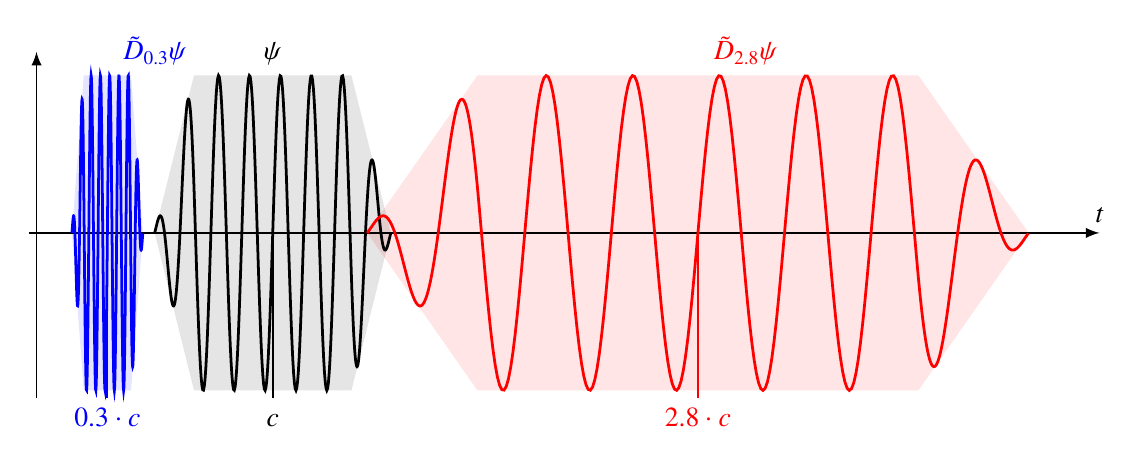
\begin{tikzpicture}[>=latex]

\def\pivalue{3.14159}

\def\bone{2.8}
\def\btwo{0.3}
\def\frequency{16}

\fill[color=gray!20] (1.5,0)--(2,-2)--(4,-2)
	--(4.5,0)--(4,2)--(2,2)--cycle;

\fill[color=blue!10] ({1.5*\btwo},0)--({2*\btwo},-2)--({4*\btwo},-2)
	--({4.5*\btwo},0)--({4*\btwo},2)--({2*\btwo},2)--cycle;
\fill[color=red!10] ({1.5*\bone},0)--({2*\bone},-2)--({4*\bone},-2)
	--({4.5*\bone},0)--({4*\bone},2)--({2*\bone},2)--cycle;

\begin{scope}
\clip (1.5,0)--(2,-2)--(4,-2)--(4.5,0)--(4,2)--(2,2)--cycle;
\definecolor{bluegray}{rgb}{0.8,0.8,0.9}
\definecolor{redgray}{rgb}{0.9,0.8,0.8}
\fill[color=bluegray] ({1.5*\btwo},0)--({2*\btwo},-2)--({4*\btwo},-2)
	--({4.5*\btwo},0)--({4*\btwo},2)--({2*\btwo},2)--cycle;
\fill[color=redgray] ({1.5*\bone},0)--({2*\bone},-2)--({4*\bone},-2)
	--({4.5*\bone},0)--({4*\bone},2)--({2*\bone},2)--cycle;
\end{scope}

\draw[->,line width=0.7pt] (-0.1,0)--(13.5,0) coordinate[label={$t$}];
\draw[->,line width=0.7pt] (0,-2.1)--(0,2.3);

%\foreach \x in {1,...,13}{
%	\draw[line width=0.7pt] ({\x},-0.1)--({\x},0.1);
%}

\node at (3,2) [above] {$\psi$};
\node[color=blue] at (1.5,2) [above] {$\tilde{D}_{\btwo}\psi$};
\node[color=red] at (9,2) [above] {$\tilde{D}_{\bone}\psi$};

\draw[line width=1pt]
	plot[domain=-1.5:-1,samples=100]
		({\x+3},{2*2*(\x+1.5)*sin(\frequency*\x*(180/\pivalue))}) --
	plot[domain=-1:1,samples=200]
		({\x+3},{2*sin(\frequency*\x*(180/\pivalue))}) --
	plot[domain=1:1.5,samples=100]
		({\x+3},{-2*2*(\x-1.5)*sin(\frequency*\x*(180/\pivalue))});

\draw[color=blue,line width=1pt]
	plot[domain=-1.5:-1,samples=100]
		({(\x+3)*\btwo},{2*2*(\x+1.5)*sin(\frequency*\x*(180/\pivalue))}) --
	plot[domain=-1:1,samples=200]
		({(\x+3)*\btwo},{2*sin(\frequency*\x*(180/\pivalue))}) --
	plot[domain=1:1.5,samples=100]
		({(\x+3)*\btwo},{-2*2*(\x-1.5)*sin(\frequency*\x*(180/\pivalue))});

\draw[color=red,line width=1pt]
	plot[domain=-1.5:-1,samples=100]
		({(\x+3)*\bone},{2*2*(\x+1.5)*sin(\frequency*\x*(180/\pivalue))}) --
	plot[domain=-1:1,samples=200]
		({(\x+3)*\bone},{2*sin(\frequency*\x*(180/\pivalue))}) --
	plot[domain=1:1.5,samples=100]
		({(\x+3)*\bone},{-2*2*(\x-1.5)*sin(\frequency*\x*(180/\pivalue))});

\draw[color=red,line width=0.7pt] ({3*\bone},0)--({3*\bone},-2.1);
\node[color=red] at ({3*\bone},-2.1) [below] {$\bone\cdot c\mathstrut$};
\draw[color=blue,line width=0.7pt] ({3*\btwo},0)--({3*\btwo},-2.1);
\node[color=blue] at ({3*\btwo},-2.1) [below] {$\btwo\cdot c\mathstrut$};
\draw[line width=0.7pt] (3,0)--(3,-2.1);
\node at (3,-2.1) [below] {$c\mathstrut$};

\end{tikzpicture}
\end{document}



%
% transdil.tex
%
% (c) 2019 Prof Dr Andreas Müller, Hochschule Rapperswil
%
\ifthenelse{\boolean{presentation}}{

\begin{frame}
\frametitle{Translation und Dilatation}
\begin{center}
\begin{tikzpicture}[>=latex]

\draw[color=blue!40,line width=1pt] plot[domain=-6:6,samples=100]
	({\x},{1.1+cos(\x*(180/3.1415))-4});

\def\bmax{101}
\pgfmathparse{0.5*(\bmax-1)}
\xdef\s{\pgfmathresult}

\foreach \b in {1,...,{\bmax}}{
	\only<\b>{
		\pgfmathparse{6*((\b)-1-\s)/(\s)}
		\xdef\B{\pgfmathresult}
		\pgfmathparse{1.1+cos(\B*180/3.1415)}
		\xdef\A{\pgfmathresult}
		\flaeche{\A}{\B}{1}
		\achsen{1.5}
		\curve{\A}{\B}{1}
		\cwt{\A}{\B}{-2.0}
	}
}

\end{tikzpicture}
\end{center}
\end{frame}

}{}








